% last updated in April 2002 by Antje Endemann
% Based on CVPR 07 and LNCS, with modifications by DAF, AZ and elle, 2008 and AA, 2010, and CC, 2011; TT, 2014; AAS, 2016

\documentclass[runningheads]{llncs}
\usepackage{graphicx}

\usepackage{amsmath,amssymb} % define this before the line numbering.
\usepackage{mathtools}
\usepackage{xfrac}

\usepackage{multirow}

\usepackage{algorithm}
\usepackage{algpseudocode}
\usepackage{ruler}
\usepackage{color}
\usepackage[width=122mm,left=12mm,paperwidth=146mm,height=193mm,top=12mm,paperheight=217mm]{geometry}
\begin{document}
% \renewcommand\thelinenumber{\color[rgb]{0.2,0.5,0.8}\normalfont\sffamily\scriptsize\arabic{linenumber}\color[rgb]{0,0,0}}
% \renewcommand\makeLineNumber {\hss\thelinenumber\ \hspace{6mm} \rlap{\hskip\textwidth\ \hspace{6.5mm}\thelinenumber}}
% \linenumbers
\pagestyle{headings}
\mainmatter
\def\ECCV16SubNumber{***}  % Insert your submission number here

\title{Incorporating Multi-Scale Analysis For Depth Estimation} % Replace with your title

\titlerunning{ECCV-16 submission ID \ECCV16SubNumber}

\authorrunning{ECCV-16 submission ID \ECCV16SubNumber}

\author{Anonymous ECCV submission}
\institute{Paper ID \ECCV16SubNumber}


\maketitle

\begin{abstract}
Convolutional neural networks exhibit exceptional performance in predicting depth from stereo images. However, this performance comes with two essential drawbacks (a) they consume extraordinary computational power (clusters of GPUs) even for a single prediction and (b) their memory and computational demand are preset from the training phase; hence they cannot be adjusted to the available resources of each application at test time.
For confronting these problems, we propose a scalable CNN architecture (MSNet) that adjusts to the specific requirements of each application; it can reduce its computational demands by sacrificing some precision or target for high accuracy if more resources are available. The bias towards accuracy or efficiency can be determined at test time, without any need for retraining. For achieving such scalability, we adopted the basic ideas of scale-space theory and incorporated them into the MSNet architecture.
MSNet exhibits challenging performance comparing to the state-of-the-art methods in the SceneFlow dataset, even though it uses considerably less learnable parameters. 

\keywords{Depth Estimation, Stereo Vision, Deep Learning, Multi-Scale Processing}
\end{abstract}

%%%%%%%%%%%%%%%%%%%%%%%%%%%%%%%%%%%%%%%%%%%%%%%%%%%%%%%%%%%%%%%%%%%%%%%%%%%%%%%%%%%%%%%%%%%%%%%%%%%%%%%%%%%%%%%%%%%%%%%%%%%%%%%%%%%%%%%%%%%%%%%%%%%
\section{Introduction}

Stereo vision forms a particular case of the general 3D reconstruction problem. Stereo cameras share the same orientation while their center is displaced horizontally by a distance $B$. The following relation expresses stereo vision's 3D geometry:

\begin{equation} \label{eq:stereo_geometry}
z = f\frac{B}{d}
\end{equation}

where $z$ is the distance from the camera level (depth), $f$ is the focal length and $d$ is the disparity. Defining the stereo pair as $X = (X^L, X^R)$, the stereo problem demotes in finding all correspondences $X^L(x,y) \leftrightarrow X^R(x-d, y) \forall (x,y)$ which, subsequently, is treated as a patch-matching procedure. Thus, disparity estimation is based on the hypothesis that the local context of correspondent points is similar. If we define as $P^{ \{L|R\} }_{n \times n}[x,y]$ the  $n \times n$ square patch centered at $X^{ \{L|R\} }[x,y]$ and $g(\cdot)$ a metric of patch similarity, then we hope that:

\begin{equation}
\begin{gathered} \label{eq:similarity_hypothesis}
    g(P^L_{n \times n}[x,y], P^R_{n \times n}[x-d^*,y]) > g(P^L_{n \times n}[x,y], P^R_{n \times n}[x-d,y]) \\
    \forall d \in [0,D] : d \neq d^*, \text{where $d* = Y[x,y]$}
\end{gathered}
\end{equation}

For hypothesis \ref{eq:similarity_hypothesis} to hold, we must choose thoughtfully two critical parameters that depend on the visual properties of the reference point: (a) the size of the surrounding area that will be incorporated (b) the scale of the comparison. Multiscale analysis provides an elegant framework for handling both the above difficulties. Furthermore, it offers the mechanism for designing a scalable CNN model.

We define as $X^{ \{L|R\} (k,q)}$ the image obtained from $X^{ \{L|R\}} \equiv X^{ \{L|R\} (k_0=1,q_0=1)}$ through the typical downscaling process:

\begin{equation}
\begin{gathered} \label{eq:downsampling_procedure}
    X^{ \{L|R\} (k_0=1,q_0=1)} \xrightarrow{downscaling} 
    X^{ \{L|R\} (k,q_0=1)} \xrightarrow{downsampling} 
    X^{ \{L|R\} (k,q)}
    \\
    k\geq 1, q\geq 1 
\end{gathered}
\end{equation}

The paramters $k \geq 1$ and $q \geq 1$ are the downscaling and downsampling rate. The downscaling part is performed with a low-pass filter (e.g. Gaussian kernel) and the downsampling through an interpolation method. Based on this formulation, we define a patch on a downscaled image as:

\begin{gather}
    P^{ \{L|R\} (k,q)}_{n \times n}[x,y] = X^{ \{ L|R \}(k,q)} [x-n:x+n, y-n:y+n]
\end{gather}

For each reference point $[x,y]$ there is a different combination of scale $k$ and patch size $n \times n$ that leads to a thriving matching procedure. For example, regions without texture require large patch size, in order to incorporate features from neighbour objects. On the other hand, for small foreground objects, a small patch is suitable, since, in this case, background objects add noise to the comparison. This variability requires the execution of the patch matching process for various combinations of scales and patch-sizes. If we define as $K$ and $N$ the set of scales and patch sizes attempted, the computational complexity of the matching becomes $O(\| K \|, \| N \|) = \| K \| \| N \|$. For maintaining low complexity, we restrict the search space in one dimension, binding $k, n$ to a single parameter $t\geq1$:

\begin{gather}
    n \times n = t(n_o \times n_0) \label{eq:t_param1}\\
    k = t \label{eq:t_param2}
\end{gather}

?? Explain why this binding ??

Due to the downscaling properties (i.e. removal of high-frequency details), it is feasible to downsampling the image without loss of information. Therefore, the two following patches contain similar information, even though they have different size:

\begin{gather} \label{eq:patch_similar_information}
    P^{ \{L|R\} (k,q=1)}_{n \times n}[x,y] \approx P^{ \{L|R\} (k,q)}_{\sfrac{(n \times n)}{q}}[\lceil \sfrac{x}{q} \rceil,\lceil \sfrac{y}{q} \rceil], \forall q \leq k
\end{gather}{}

Due to equation \ref{eq:patch_similar_information} it is feasible to obtain similar patch matching curves, if instead of increasing the patch size, we downsample the stereo pair:

\begin{gather} \label{eq:patch_similar_information1}
     P^{ \{L|R\} (k = t, q = t)}_{(n_0 \times n_0)}[\lceil \sfrac{x}{t} \rceil, \lceil \sfrac{y}{t} \rceil] \approx P^{ \{L|R\} (k = t, q = 1)}_{t(n_0 \times n_0)}[x,y] 
\end{gather}{}

In figure \ref{fig:multiscale_importance_2D}, we design a simple artificial example to underline the importance of multiscale processing. We draw two different test cases: in the left-column scenario the fine-scale ($k=1$) with a small patch size ($n_0 \times n_0 = 5 \times 5$) leads to superior accuracy, whereas in the right-column scenario the coarse-scale ($k=t=2.6$) with larger patch size ($t(n_0 \times n_0) = 2.6(5 \times 5) =13 \times 13$) is a better fit. In both cases, the matching score curve is similar for using $ P^{ \{L|R\} (k = 2.6, q = 1)}_{13 \times 13}[x,y] $ (red curve) and $P^{ \{L|R\}, (k = 2.6, q = 2.6)}_{5 \times 5}[\lceil \sfrac{x}{2.6} \rceil, \lceil \sfrac{y}{2.6} \rceil ]$ (green curve), confirming the claim of equation \ref{eq:patch_similar_information1}.

\begin{figure}[!t]
    \begin{center}
        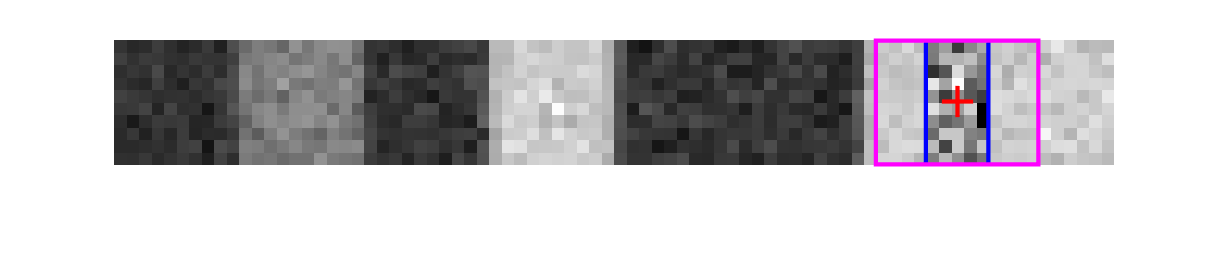
\includegraphics[width=0.49\textwidth]{figures/high_resolution_success_imL_fine.png}
        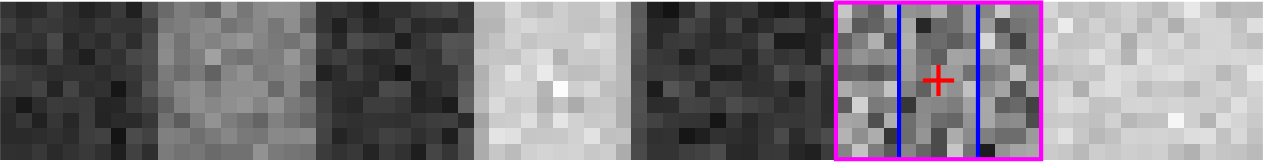
\includegraphics[width=0.49\textwidth]{figures/low_resolution_success_imL_fine.png}\\
        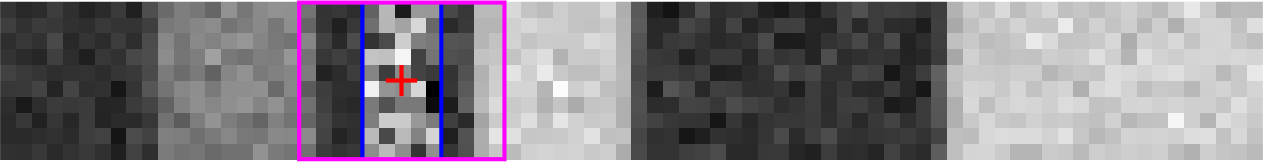
\includegraphics[width=0.49\textwidth]{figures/high_resolution_success_imR_fine.png}
        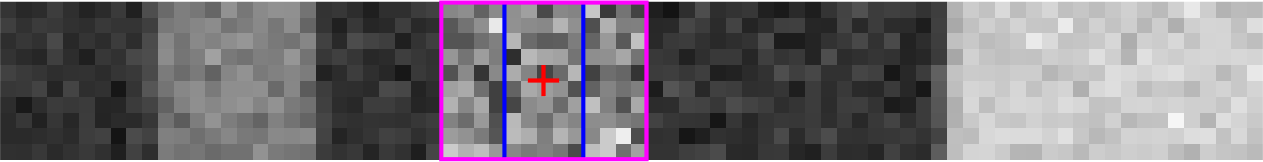
\includegraphics[width=0.49\textwidth]{figures/low_resolution_success_imR_fine.png}\\
        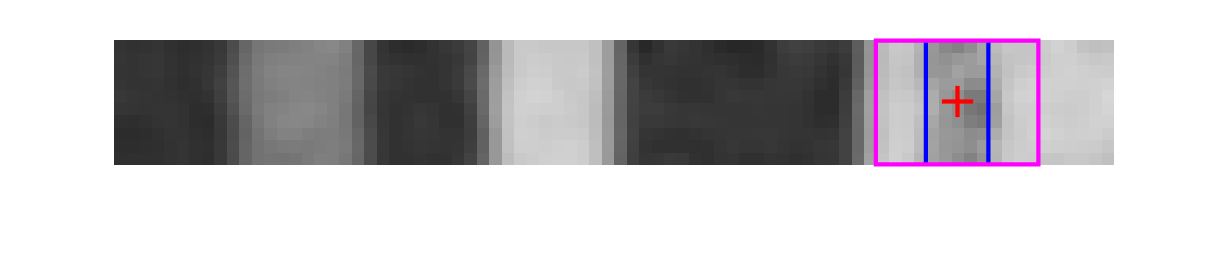
\includegraphics[width=0.49\textwidth]{figures/high_resolution_success_imL_coarse.png}
        
\includegraphics[width=0.49\textwidth]{figures/low_resolution_success_imL_coarse.png}\\
        
\includegraphics[width=0.49\textwidth]{figures/high_resolution_success_imR_coarse.png}
        
\includegraphics[width=0.49\textwidth]{figures/low_resolution_success_imR_coarse.png}\\
        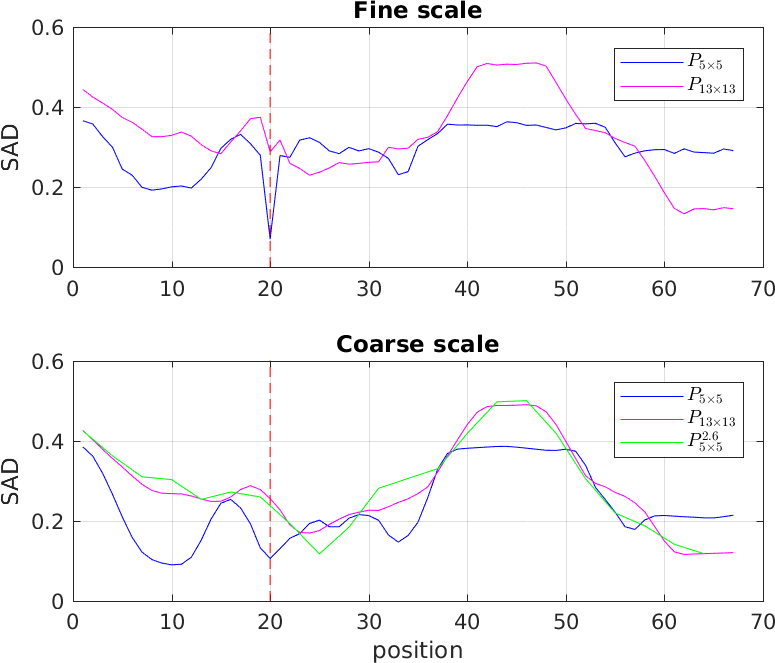
\includegraphics[width=0.49\textwidth]{paper/latex/figures/high_resolution_success_graph.png}
        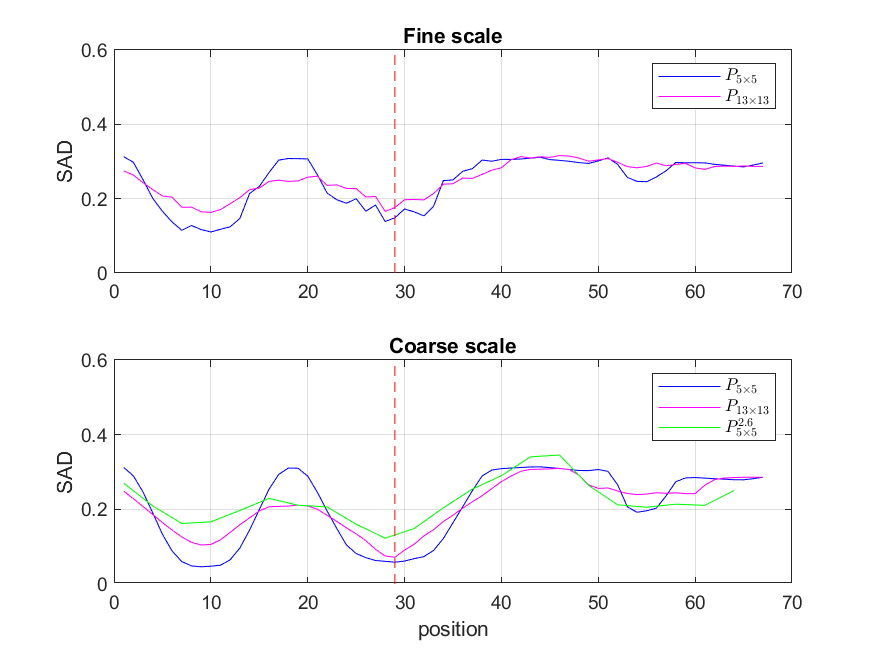
\includegraphics[width=0.49\textwidth]{paper/latex/figures/low_resolution_success_graph.png}\\
        
    \end{center}
    
    \caption{Simple artificial example. The left and the right column correspond to two different scenarios. In both columns, the first two images are the left and the right stereo view of the same 3D pattern, using orthographic projection. The next two images are the same views downscaled by a Gaussian filter. The red and blue bounding box corresponding to the two different patch sizes and the red cross to the reference point. In the graphs, we observe the curves of the matching process. The red dotted vertical line corresponds to the ground truth disparity.}
    \label{fig:multiscale_importance_2D}
\end{figure}

!!Apart from improving the patch matching procedure, the multiscale analysis provides the tools for designing an agile CNN architecture that can be readjusted between efficiency and accuracy at test time (i.e. without repeating the training procedure). The learnable parts of the CNN can be repeated between the processing scales that are set at the test phase. Thus, if we seek for efficiency and a rough estimation of the depth, we can tune the network to operate on coarse scales; conversely, if accuracy is the priority, we can set the network to fine scales, leading to more detailed prediction.!!
%%%%%%%%%%%%%%%%%%%%%%%%%%%%%%%%%%%%%%%%%%%%%%%%%%%%%%%%%%%%%%%%%%%%%%%%%%%%%%%%%%%%%%%%%%%%%%%%%%%%%%%%%%%%%%%%%%%%%%%%%%%%%%%%%%%%%%%%%%%%%%%%%%%

\section{Related Work}

Reconstructing the three dimensional geometry from a set of $2D$ images is a core problem of computer vision. Stereo reconstruction is a predominant technique of the aforementioned domain and has been heavily studied over years \cite{Barnard1982ComputationalStereo},\cite{Brown2003}. Scharstein and Szeliski \cite{Scharstein2001AAlgorithms} propose a general taxonomy framework for describing and analysing any stereo vision algorithm in four steps: matching cost computation, cost aggregation, disparity computation/optimisation and disparity refinement.

The matching cost computation realises a dissimilarity measurement between each pixel on reference image and all possible corresponding locations. Quite a lot of metrics of dissimilarity have been proposed, including  absolute difference, squared difference, cross correlation and hamming distance. Dissimilarity metrics can be applied on many different local descriptors, such as LoG, CENSUS \cite{Zabih1996ACorrespondence} and BRIEF \cite{Calonder2010}. Mutual Information \cite{Viola1997} proposes a rather different metric based on the entropy of histograms of correnspondent locations. An extensive evaluation of different matching cost computation strategies has been proposed by \cite{Hirschmuller2007}. Initial matching costs are error prone due to the intense locality of information. Initial estimates need to get optimized by methods taking into account global image information. This can be accomplished through graph cuts \cite{Kolmogorov}, \cite{Boykov2001} and belief propagation \cite{Klaus2006}. Semi-Global-Matching (SGM) \cite{Hirschmuller2008StereoInformation} attempts to minimize a global energy function.

Stereo vision methods are evaluated on datasets containing ground truth depth or disparity for stereo pairs. Middlebury \cite{Scharstein2014} contains indoor scenes. KITTI \cite{Menze2015ISA}, \cite{Menze2018JPRS} is a larger dataset with outdoor scenes and ground truth labels collected from LIDAR on a moving vehicle. Mayer et. al \cite{Mayer2016ALD} created a big synthetic dataset for training big machine learning models.

Deep convolutional networks show great success on stereo vision problems. Intial deep learning proposals focused on matching cost compuation. Zagoruyko et. al \cite{Zagoruyko2015LearningNetworks} proposed a deep convolutional neural network for comparing image patches. \v{Z}bontar and LeCun \cite{Zbontar_2015_CVPR} trained a deep network for predicting the initial matching scores on $9x9$ image patches, followed by traditional aggregation and refinement methods. Luo et. al \cite{Luo2016EfficientMatching} treated matching scores estimation as a multi-label classification problem.

Shaked and Wolf [12] introduce an initial disparity prediction network pooling global information from cost volume

%%%%%%%%%%%%%%%%%%%%%%%%%%%%%%%%%%%%%%%%%%%%%%%%%%%%%%%%%%%%%%%%%%%%%%%%%%%%%%%%%%%%%%%%%%%%%%%%%%%%%%%%%%%%%%%%%%%%%%%%%%%%%%%%%%%%%%%%%%%%%%%%%%%
\section{Our Model}

In this section we analyse the building blocks (modules) that comprise the proposed MultiScaleNetwork (MSNet). We name each module as $m_i$; its learnable part as $f_i$ and the non-learnable part as $g_i$. Some modules contain only learnable parts and other only non-learnable. In all cases, the learnable parts are CNNs. All modules are differentiable so that the backpropagation algorithm to be applicable end-to-end. Figure \ref{fig:cnn_architecture} provides a visual graph of the end-to-end architecture.

\begin{figure}[!htbp]
    \centering
    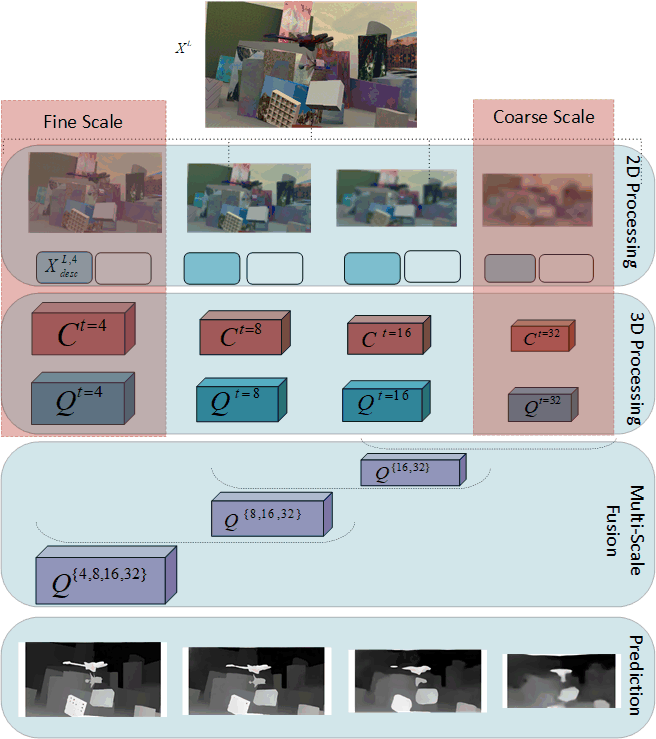
\includegraphics[width=0.7\textwidth]{figures/stereo_architecture.png}
    \caption{Scale fusion network overview. Its main constructive blocks are the horizontal pipelines (green colour) representing end-to-end predictions at specific scale $\sigma$ and the vertical pipelines (grey colour) representing the pair-scales fusion at similarity matrix level. The red-coloured blocks are the learned parts of our architecture, while the yellow coloured ones are hand-crafted layers.}
    \label{fig:cnn_architecture}
\end{figure}

% \begin{table}
%     \centering
%     \begin{tabular}{ l|c|c }
%     Description & Symbol & Set \rule{0pt}{2ex}\\
    
%     \hline
%     \multicolumn{3}{c}{ \textbf{Definitions} } \rule{0pt}{2.4ex}\\
%     \hline
    
%     Raw image & $X^L, X^R$ & $\mathbb{R}^{H \times W \times 3}$ \rule{0pt}{2.5ex} \\
    
%     Ground truth & $Y$ & $\mathbb{R}^{H \times W}$ \rule{0pt}{2.5ex} \\
    
%     \hline
%     \multicolumn{3}{c}{ \textbf{Single-Scale 2D Processing} } \rule{0pt}{2.4ex}\\
%     \hline
    
%     Downscaled image & $X^{L,t}, X^{R, t}$ & $\mathbb{R}^{\sfrac{H}{t} \times \sfrac{W}{t} \times 3}$ \rule{0pt}{3ex} \\
    
%     Descriptor image at scale $t$ & $X^{L,t}_{desc}, X^{R, t}_{desc}$ & $\mathbb{R}^{\sfrac{H}{t} \times \sfrac{W}{t} \times K}$ \rule{0pt}{3.5ex} \rule[-1.3ex]{0pt}{0pt}\\
    
%     \hline
%     \multicolumn{3}{c}{ \textbf{Single-Scale 3D Processing} } \rule{0pt}{2.4ex}\\
%     \hline
    
%     Comparison volume & $C^{t}$ & $ \mathbb{R}^{ \sfrac{D}{t} \times \sfrac{H}{t} \times \sfrac{W}{t} \times K } $ \rule{0pt}{3ex} \\
    
%     Processed comparison volume & $Q^{t}$ & $ \mathbb{R}^{ \sfrac{D}{t} \times \sfrac{H}{t} \times \sfrac{W}{t} \times K } $ \rule{0pt}{3ex} \\
    
%     Similarity volume & $S^{t}$ & $ \mathbb{R}^{ \sfrac{D}{t} \times \sfrac{H}{t} \times \sfrac{W}{t}} $  \rule{0pt}{3.5ex} \\
    
%     Prediction image & $\hat{Y}^{t}$ & $\mathbb{R}^{H \times W}$ \rule{0pt}{3.5ex} \\
    
%     \hline
%     \multicolumn{3}{c}{ \textbf{Multi-Scale 3D Processing} } \rule{0pt}{2.4ex} \\
%     \hline
    
%     Processed comparison volume & $Q^{ \{ t_0, ... , t_n \} }$ & $ \mathbb{R}^{ \sfrac{D}{t_0} \times \sfrac{H}{t_0} \times \sfrac{W}{t_0} \times K }  $ \rule{0pt}{3ex} \\
    
%     Similarity volume & $S^{ \{ t_0, ... , t_n \} }$ & $ \mathbb{R}^{ \sfrac{D}{t_0} \times \sfrac{H}{t_0} \times \sfrac{W}{t_0}} $ \rule{0pt}{3.5ex} \\
    
%     Prediction image & $\hat{Y}^{ \{ t_0, ... , t_n \} }$ & $\mathbb{R}^{ H \times W}$ \rule{0pt}{3.5ex} \\
%     \hline
%     \end{tabular}
%     \caption{Description of all tensors involved in MSNet. All tensors follow the dimensions defined by their scale, apart from the final prediction image $\hat{Y}$. In this case, the scale (or list of scales) declares the processing scales used in the prediction. The final prediction shares always the same dimension as the raw images.}
%     \label{tab:entity_description}
% \end{table}

\subsubsection{Downscaling Module - $m_1^t$}

The module $m_1^t: \mathbb{R}^{H \times W} \rightarrow \mathbb{R}^{\lceil \sfrac{H}{t} \rceil \times \lceil \sfrac{W}{t} \rceil }$ creates a downscaled stereo pair by being applied separately in each stereo image: 

\begin{equation} \label{eq:g1}
    (X^{L,t}, X^{R,t}) = (m_1^t(X^L), m_1^t(X^R))
\end{equation}{}

The parameter $t$ is the downscaling and downsampling factor, as defined in equations \ref{eq:t_param1}, \ref{eq:t_param2}. The $m_1^t$ is a two-step procedure; firstly each stereo image $X^{\{L|R\}}$ is convolved with the discrete Gaussian kernel of equation \ref{eq:g1_kernel} in order to remove the high-frequency components, and subsequently a bilinear downsampling is applied:

\begin{gather} \label{eq:g1_kernel}
    k(x, y, \sigma) = \frac{1}{2\pi\sigma^2} \cdot e^{\sfrac{-(x^2 + y^2)}{2\sigma^2}} \\
    x,y \in \{-\lceil 4*\sigma + 0.5 \rceil, ..., \lceil 4*\sigma + 0.5 \rceil\}, \sigma = \sfrac{t}{3}
\end{gather}

\subsubsection{Feature Extraction - $m_2$}

The module $m_2: \mathbb{R}^{H \times W \times 3} \rightarrow \mathbb{R}^{H \times W \times K}$ extracts local features from the raw stereo images, through a CNN $f_2$. The feature extraction process is repeated separately at each scale:

\begin{equation} \label{eq:f_1}
    m_2:(X^{L,t}_{desc}, X^{R,t}_{desc}) = (f_2(X^{L,t}), f_2(X^{R, t}))
\end{equation} 

\subsubsection{Comparison Volume - $m_3$} The module $m_3$
$$m_3:(\mathbb{R}^{H \times W \times K}, \mathbb{R}^{H \times W \times K}, \mathbb{R}^{H \times W \times 3}) \rightarrow \mathbb{R}^{D \times H \times W \times (K+3)}$$ forms the Comparison Volume $C^t$, by zipping the comparison information into a 3D tensor. Normally, the Comparison Volume is formed by simply concatenating the descriptors in each disparity position. This approach introduces significant redundancy: from the $D \times H \times W \times 2K$ values of the Comparison Volume only the $H \times W \times 2K$ are unique. For reducing such redundancy, we design a new comparison metric between two scalar features:

\begin{equation} \label{eq:m}
    l: \mathbb{R}^2 \rightarrow \mathbb{R}: l(a_1, a_2) = \frac{|a_1| + |a_2|}{2} \cdot e^{-|a_1 - a_2|}    
\end{equation}

 The first term $\frac{|a_1| + |a_2|}{2}$ measures the existence of a feature in each patch separately ($0$ signifies non-existence) and the second term $e^{-|a_1 - a_2|} \in (0,1]$ measures the coexistence of the feature in both patches. Finally, we concatenate the raw left image $X^L$, in order to propagate the raw image in the subsequent layers. The formulation of the comparison volume is described in equation \ref{eq:comparison_volume}:

\begin{equation}\label{eq:comparison_volume}
C^t[d, x, y, i] = 
    \begin{cases}
        l( X^{L, t}_{desc}[x,y,i], X^{R, t}_{desc}[x-d,y, i]) &\quad ,i \leq K \\
        X^{L,t}[x,y,i-K] &\quad ,i > K
     \end{cases}
\end{equation}{}  


\subsubsection{Comparison Volume Processing - $m_4$} The module $m_4: \mathbb{R}^{D \times H \times W \times K} \rightarrow \mathbb{R}^{D \times H \times W \times K}$ is a CNN ($f_4$) with 3D convolutional layers, that incorporates local information along all 3 dimensions (the 2 spatial ones $x,y$ and the disparity $d$) for refining the Comparison Volume. It ouptuts a same-dimension volume $Q^t$:

\begin{equation}
    m_4: Q^t = f_4(C^t)
\end{equation}


\subsubsection{Multiscale Fusion - $m_5$}

This module is responsible for exploiting information from different scales and combine it in a single tensor. The procedure takes place recursively in pairs of two Comparison Volumes, from coarse to fine scales. A trilinear upsampling layer $g_3^t: \mathbb{R}^{D \times H \times W \times K} \rightarrow \mathbb{R}^{tD \times tH \times tW \times K}$ is applied to the low-dimension Comparison Volume before a CNN ($f_5$) with 3D-Convolutional layers implement the learning procedure:

\begin{equation} \label{eq:two_scale_fusion}
Q^{ \{ t_i, \cdot \cdot \cdot, t_{n} \} } = f_5(Q^{t_i} \oplus g_5^{\sfrac{t_i}{t_{i-1}} }(Q^{ \{ t_{i-1}, \cdot \cdot \cdot, t_n \} }))
\end{equation}

In Algorithm \ref{alg:multi_scale_fusion} we present the Multi-scale fusion method end-to-end. The upsampling and the merging procedure are applied sequentially from coarse-to-fine scale, leading to a Comparison Volume $Q^{\{t_0, t_1, \cdot \cdot \cdot, t_n\}}$ with combined information from all scales.

\begin{algorithm}
\caption{Multi-scale fusion - Module $m_5$}\label{alg:multi_scale_fusion}
\begin{algorithmic}[1]
\Procedure{multi scale fusion}{$ Q^{t_0}, Q^{t_1}, \cdot \cdot \cdot, Q^{t_n} $} $\rightarrow Q^{\{t_0, t_1, \cdot \cdot \cdot, t_n\}}$ 
\State $Q \gets Q^{t_n}$ \Comment{Initialize}
\For { \texttt{i=n-1;-1;0} }
\State $Q \gets g_3^{\sfrac{ t_{i+1} }{ t_i } }(Q)$ \Comment{3D Upsampling}
\State $Q \gets Q^{t_i} \oplus Q$ \Comment{Concatenation}
\State $Q \gets f_5(Q)$ \Comment{Merge information}
\EndFor
\State \Return $Q^{\{t_0, t_1, \cdot \cdot \cdot, t_n\}} \gets Q$ \Comment{Result}
\EndProcedure
\end{algorithmic}
\end{algorithm}


\subsubsection{Module For Depth Prediction - $m_6$}

The module $m_6^t: \mathbb{R}^{\sfrac{D}{t} \times \sfrac{H}{t} \times \sfrac{W}{t} \times K} \rightarrow \mathbb{R}^{D \times H \times W}$ implements the depth prediction. It consists of three sequential parts: (a) a CNN with 3D-convolutional layers $f_6: \mathbb{R}^{D \times H \times W \times K} \rightarrow \mathbb{R}^{D \times H \times W}$ that assigns a probability in each possible disparity $S^{\{ t_0, \cdot \cdot \cdot, t_n \}} = f_6(Q^{\{t_0, t_1, \cdot \cdot \cdot, t_n\}})$, (b) a trilinear upsampling layer for upsampling $S$ in the initial dimensions $D \times H \times W$ and finally (c) a softmax operator applied along the disparity dimension, for obtaining the final prediction $\hat{Y}^{\{t_0, t_1, \cdot \cdot \cdot, t_n\}}$.

\subsubsection{Putting all pieces together}

The MSNet has 4 different learnable CNNs - $f_2, f_4, f_5, f_6$, inside the 5 modules. The modules $m_1, m_2, m_3$ operate repeatedly at each separate scale and the modules $m_4, m_5$ produce the final prediction by incorporating information from all scales. At training phase, we set the set of scales to be $T = \{ 2^2, 2^3, 2^4, 2^5 \}$. At test time, as mentioned before, the set of processing scales can change arbitrarily. For example, if the application lacks computational resources and targets to a quick depth estimation $T$ can be set to $\{ 16, 32, 64\}$, whereas if the application needs accuracy and high-resolution detail $T = \{1, 2, 4, 8, 16, 32, 64 \}$ is a better choice. In the next section, we present experimental results on how the accuracy changes among different sets of scales. The complete MSNet method can be summarized in the following steps:


\begin{algorithm}
\caption{MultiScaleNetwork (MSNet)}\label{alg:MSNET}
\begin{algorithmic}[1]
\State $T \gets \{ t_0, t_1, ... , t_n\}$ \Comment{Define Processing Scales}
\Procedure{MSNet}{$ X^L, X^R, T$} $\rightarrow \hat{Y}$ 
\For { \texttt{t in T} }
\State $(x^{L,t},  x^{R,t}) \gets (m_1^t(X^L),m_1^t(X^R)) $ \Comment{Downscaling}
\State $(x^{L,t}_{desc}, x^{R,t}_{desc}) \gets (m_2(X^L), m_2(X^L))$ \Comment{Features}
\State $C^{t} \gets m_3(X^{L,t}_{desc}, X^{R,t}_{desc}, X^{L,t})$ \Comment{Comparison Volume}
\State $Q^{t} \gets m_4(C^{t})$ 
\EndFor
\State $Q^{\{t_0, t_1, \cdot \cdot \cdot, t_n\}} \gets m_5(Q^{t_0}, Q^{t_1}, \cdot \cdot \cdot, Q^{t_n})$ \Comment{MultiScaleFusion}
\State $\hat{Y}^{\{ t_0, \cdot \cdot \cdot, t_n \}} = m_6(Q^{\{t_0, t_1, \cdot \cdot \cdot, t_n\}}) $ \Comment{Prediction}
\State \Return $\hat{Y}^{\{ t_0, \cdot \cdot \cdot, t_n \}} $
\EndProcedure
\end{algorithmic}
\end{algorithm}


% \begin{equation}
% \begin{gathered} \label{eq:full_MSNet_model}
%     (X^{L,t_i}, X^{R,t_i}) = (m_1^{t_i}(X^L), m_1^{t_i}(X^R)), \forall t_i \in T 
%     \\
%     (X^{L,t_i}_{desc}, X^{R,t_i}_{desc}) = (m_2(X^{L,t_i}), m_2(X^{R, t_i})), \forall t_i \in T 
%     \\
%     C^{t_i} = m_3(X^{L,t_i}_{desc}, X^{R,t_i}_{desc}, X^{L,t_i}), \forall t_i \in T 
%     \\
%     Q^{t_i} = m_4(C^{t_i}), \forall t_i \in T 
%     \\
%     Q^{\{t_0, t_1, \cdot \cdot \cdot, t_n\}} = m_5(Q^{t_0}, Q^{t_1}, \cdot \cdot \cdot, Q^{t_n}) 
%     \\
%     Y^{\{ t_0, \cdot \cdot \cdot, t_n \}} = m_6(Q^{\{t_0, t_1, \cdot \cdot \cdot, t_n\}}) 
%     \\
% \end{gathered}
% \end{equation}


\subsection*{Cnn architectures}

The learnable parts of MSNet ($f_2, f_4, f_5, f_6$) are four CNNs, that follow similar architecture. A residual connection is used as a fundamental building block in all architectures. The residual block comprises of two blocks of Batch Normalization, ReLU and Convolution in sequential order, with a residual connection added to the output. For the $f_2$, which operates on 2D inputs, the convolution is 2D (i.e. kernel with spatial dimension 3x3), whereas for $f_4, f_5, f_6$ the convolution is 3D, applied along the disparity dimension as well (kernel dimension 3x3x3). The table \ref{tab:learnable_models} summarizes the architectures used in each CNN.


\begin{table}[!htbp]
    \centering
    \begin{tabular}{ c|c|c|c|c|c }
    \textbf{Module} & \textbf{Structure} & \textbf{Input} & \textbf{Output} & \textbf{Parameters} & \textbf{Complexity} \\
    
    \hline
    
    \multirow{2}{*}{$f_2$} & BN+ReLU+Conv2D & HxWx3 & HxWx32 & \multirow{2}{*}{74592} & \multirow{2}{*}{O(HW)} \\
    & 4xRes2D & HxWx32 & HxWx32 & &
    \\

    \hline

    \multirow{2}{*}{$f_4$} & BN+ReLU+Conv3D & DxHxWx64 & DxHxWx32 & \multirow{2}{*}{196128} & \multirow{2}{*}{O(DHW)} \\
    & 3xRes3D & DxHxWx32 & DxHxWx32 & & \\
    
    \hline
    
    \multirow{3}{*}{$f_5$} & BN+ReLU+Conv3D & DxHxWx64 & DxHxWx64 & 
    \multirow{3}{*}{331776} & \multirow{3}{*}{O(TDHW)} \\
    & BN+ReLU+Conv3D & DxHxWx64 & DxHxWx32 & & \\
    & 3xRes3D & DxHxWx32 & DxHxWx32 & & \\

    \hline
    
    \multirow{3}{*}{$f_6$} & BN+ReLU+Conv3D & DxHxWx64 & DxHxWx64 &
    \multirow{3}{*}{139104} & \multirow{3}{*}{O(DHW)} \\
    & 2xRes3D & DxHxWx32 & DxHxWx32 & & \\
    & BN+ReLU+Conv3D & DxHxWx32 & DxHxW & & \\

    \hline
    MSNet & & HxWx3 & HxW & 741600 & O(TDHW) \\
       
    
    \end{tabular}
    \caption{Description of CNN architectures}
    \label{tab:learnable_models}
\end{table}

%%%%%%%%%%%%%%%%%%%%%%%%%%%%%%%%%%%%%%%%%%%%%%%%%%%%%%%%%%%%%%%%%%%%%%%%%%%%%%%%%%%%%%%%%%%%%%%%%%%%%%%%%%%%%%%%%%%%%%%%%%%%%%%%%%%%%%%%%%%%%%%%%%%
\section{Experimental Evaluation}

\begin{table}[!htbp]
    \centering
    \begin{tabular}{ c|c|c|c|c }
    Method & Parameters (M) & Runtime & MAE & PCG \\
    
    \hline
    \multicolumn{5}{c}{ \textbf{Our benchmark - IMS architectures} } \\
    \hline
    MSNet & 0.741 & 0.32 & 1.017 & 3.98 \\
    \hline
    OneRes (S) & 0.463 & 0.11 & 1.508 & 6.11 \\
    MRes2d (S) & 0.659 & 0.10 & 1.671 & 6.98 \\
    MRes3d (S) & 0.514 & 0.15 & 1.504 & 5.86 \\
    MRes2d3d (S) & 0.677 & 0.3 & 1.897 & 8.078 \\
    \hline
    OneRes (B) & 1.608 & 0.22 & 1.37 & 5.53 \\
    MRes2d (B) & 1.458 & 0.17 & 1.32 & 5.43 \\
    MRes3d (B) & 1.682 & 0.21 & 1.322 & 5.11 \\
    MRes2d3d (B) & 1.772 & 0.32 & 1.613 & 6.67 \\
    \hline
    \multicolumn{5}{c}{ \textbf{Our benchmark - Free weights} } \\
    \hline
    Free2d & 0.969 & 0.24 & 1.126 & 4.33 \\
    Free3d & 2.75 & 0.33 & \textbf{0.882} & \textbf{3.48} \\
    Free2d3d & 2.974 & 0.33 & 1.107 & 4.36 \\
    \hline
    \multicolumn{5}{c}{ \textbf{SOTA} } \\
    \hline
    PSMNet\cite{Chang2018PyramidNetwork} & - & - & 1.09 & - \\
    CRL\cite{Pang2018CascadeMatching} & - & - & 1.32 & - \\
    DispNetC\cite{Mayer2016ALD} & - & - & 1.68 & - \\
    GC-Net\cite{Kendall2017End-to-EndRegression} & 3.5 & 0.95 & 2.51 & 9.34 \\
    Edge-Stereo\cite{SongEdgeStereoResidual} & - & - & 1.12 & 4.99 \\
    CSPN\cite{cheng2018learning} & - & - & 0.78 & - \\
    GA-Net\cite{zhang2019ga} & 2.3 & 1.5 & 0.84 & - \\
    AMNet\cite{du2019amnet} & 4.37 & - & \textbf{0.74} & - \\
    
    \hline
    \end{tabular}
    \caption{Model comparison on SceneFlow dataset}
    \label{tab:results}
\end{table}

\begin{figure}[!htbp]
    \begin{center}
        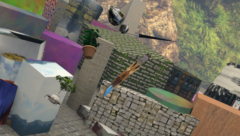
\includegraphics[width=0.24\textwidth,clip]{figures/imL_0.png}
        
\includegraphics[width=0.24\textwidth,clip]{figures/imL_1.png}
        
\includegraphics[width=0.24\textwidth,clip]{figures/imL_2.png}
        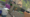
\includegraphics[width=0.24\textwidth,clip]{figures/imL_3.png}
        \\
        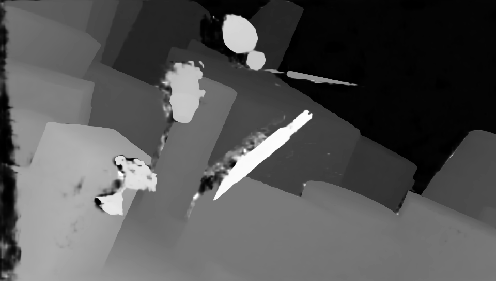
\includegraphics[width=0.24\textwidth,clip]{figures/pred_0.png}
        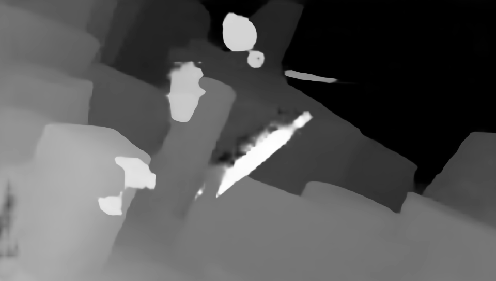
\includegraphics[width=0.24\textwidth,clip]{figures/pred_1.png}
        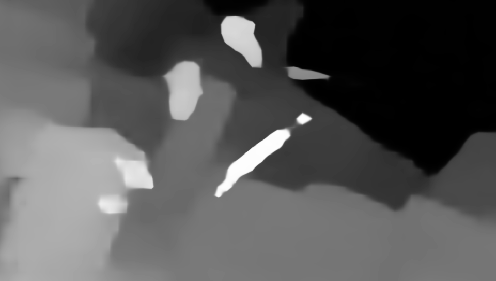
\includegraphics[width=0.24\textwidth,clip]{figures/pred_2.png}
        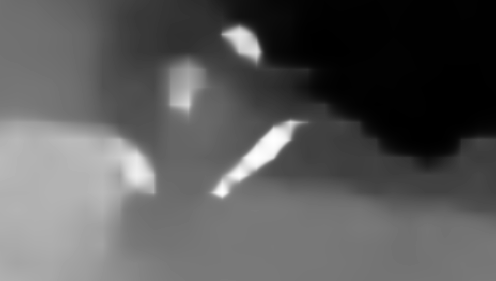
\includegraphics[width=0.24\textwidth,clip]{figures/pred_3.png}
        \\
        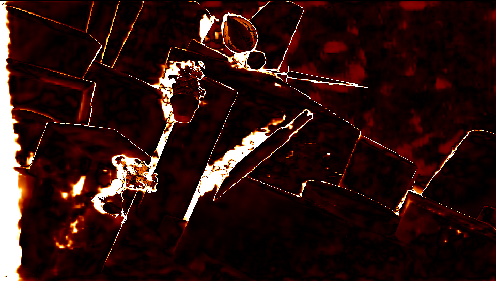
\includegraphics[width=0.24\textwidth,clip]{figures/pred_0_err.png}
        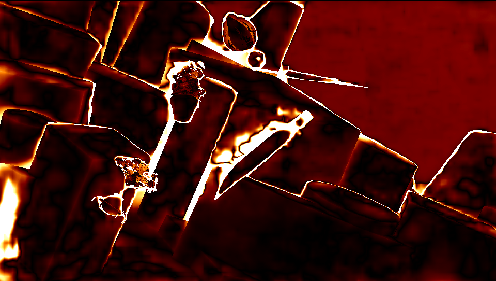
\includegraphics[width=0.24\textwidth,clip]{figures/pred_1_err.png}
        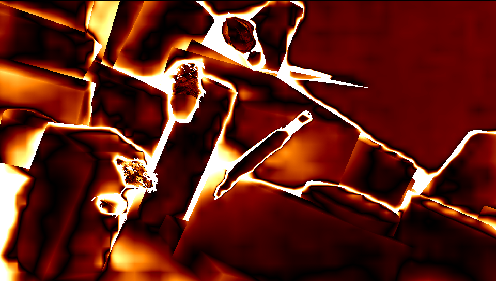
\includegraphics[width=0.24\textwidth,clip]{figures/pred_2_err.png}
        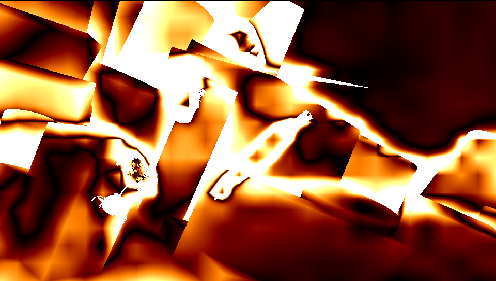
\includegraphics[width=0.24\textwidth,clip]{figures/pred_3_err.png}
        \\
        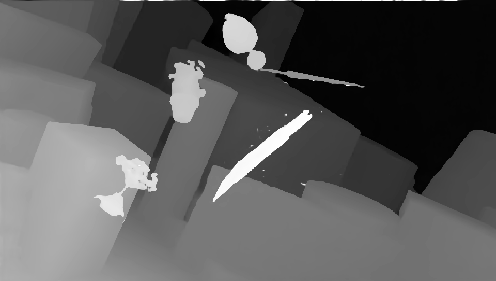
\includegraphics[width=0.24\textwidth,clip]{figures/pred_comb_0.png}
        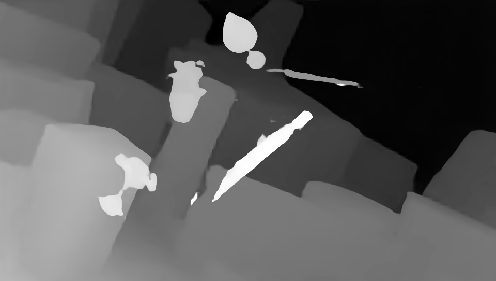
\includegraphics[width=0.24\textwidth,clip]{figures/pred_comb_1.png}
        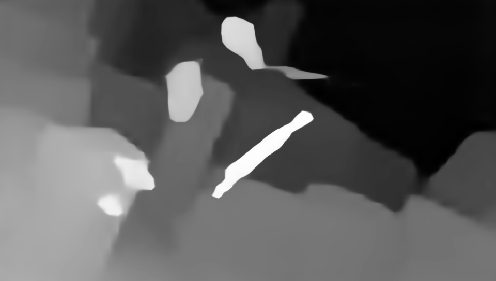
\includegraphics[width=0.24\textwidth,clip]{figures/pred_comb_2.png}
        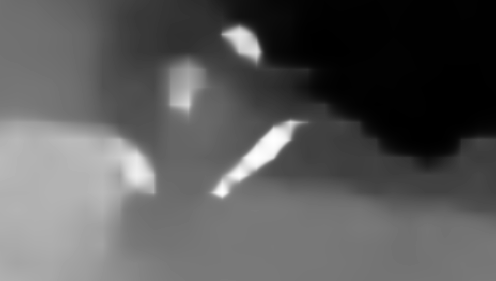
\includegraphics[width=0.24\textwidth,clip]{figures/pred_comb_3.png}
        \\
        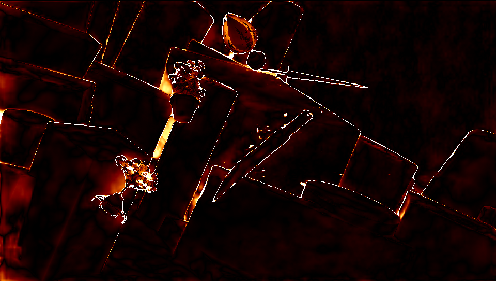
\includegraphics[width=0.24\textwidth,clip]{figures/pred_comb_0_err.png}
        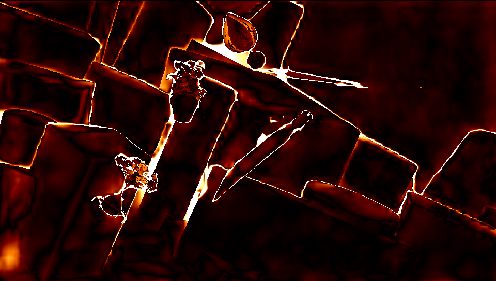
\includegraphics[width=0.24\textwidth,clip]{figures/pred_comb_1_err.png}
        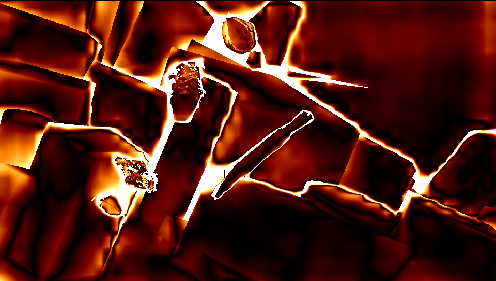
\includegraphics[width=0.24\textwidth,clip]{figures/pred_comb_2_err.png}
        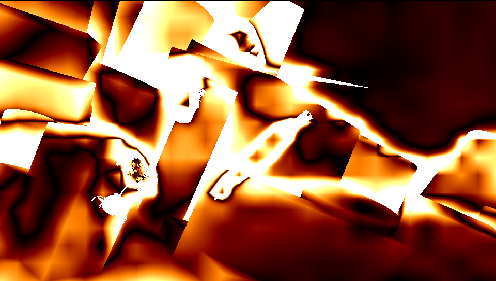
\includegraphics[width=0.24\textwidth,clip]{figures/pred_comb_3_err.png}
    \end{center}
    \caption{Analytic illustration of a prediction process. The first row (left to right) contains the left image along all scales $X^{L,t} : t \in \{2^2, 2^3, 2^4, 2^5\}$. The second and third row contain the single scale predictions $\hat{Y}^{L,t}$ and the corresponding error images $E^{L,t}$. The fourth and fifth row contains the multiscale predictions (processing scales are added as we move from right to left) and the corresponding error images. We can observe the limitations of single-scale predictions; coarse scales fail in describing the details between objects while fine scales suffer from instabilities. On the other hand, the multiscale prediction combines the benefits of both worlds; it starts with a rough estimation of the disparity image and it adds higher-resolution details as it visits fine scales.}
    \label{fig:EMAPs}
\end{figure}

In this section we measure the performance of the proposed method on the large synthetic SceneFlow dataset. Table \ref{tab:results} presents the aggregated results of our experiments and figure \ref{fig:EMAPs} the results on a single training example.

\subsection{The Effect Of Using Multi-Scale Processing Explicitly}

In this section, we test whether enforcing multi-scale processing explicitly, as in MSNet, is more beneficial than using multi-scale processing internally as part of the CNN architecture. For this reason, we design 4 new CNN models that follow the MSNet designing principles, but without enforcing multi-scale processing explicitly; Instead, we use the hourglass model (i.e. encoder-decoder architecture) which is the proposed method by the literature, for applying multi-resolution processing internally. We design the following 4 architectures; OneRes operates only on the initial resolution, MRes2d uses the hourglass model only in the 2D-processing part, MRes3d only in the 3D-processing part and finally MRes2d3d in both the 2D and 3D processing part. For each of the 4 CNNs we create two versions; the small (S) version has the same number of free parameters as MSNet and the big (B) one which has as many parameters as the memory of the GPU allows. For clarity, we call all these new models with the common name Implicit Multi-Scale (IMS) architectures.

In figure \ref{fig:mae_SFNvsGenericNets} we observe that MSNet outperforms both versions of the IMS architectures, which is a crucial indicator that enforcing multi-scale processing explicitly is beneficial for depth estimation. As expected, big (B) networks outperform small (S) ones.

\begin{figure}[!htbp]
    \centering
    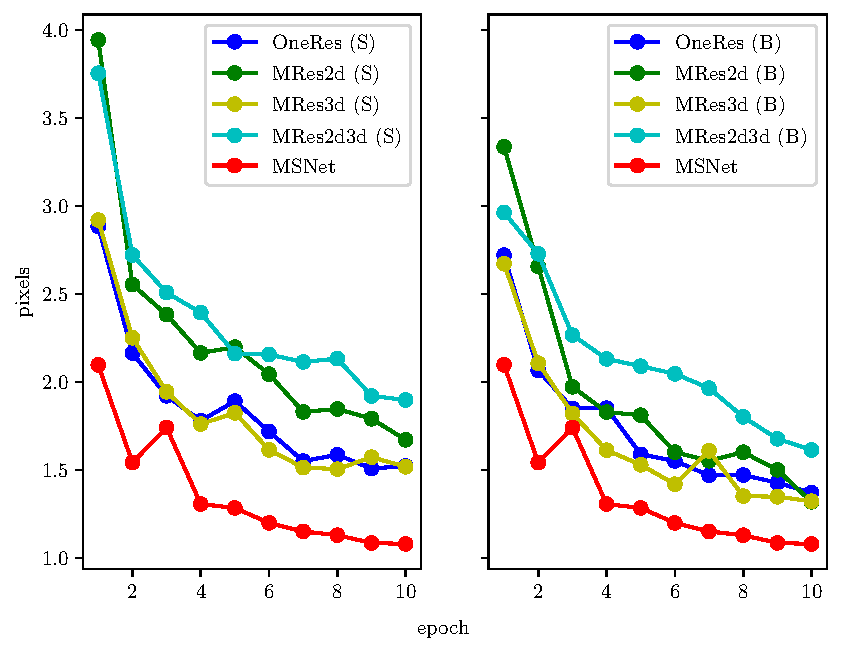
\includegraphics[width=0.49\textwidth]{figures/freiburg_msnet_vs_monolithic_mae.pdf}
    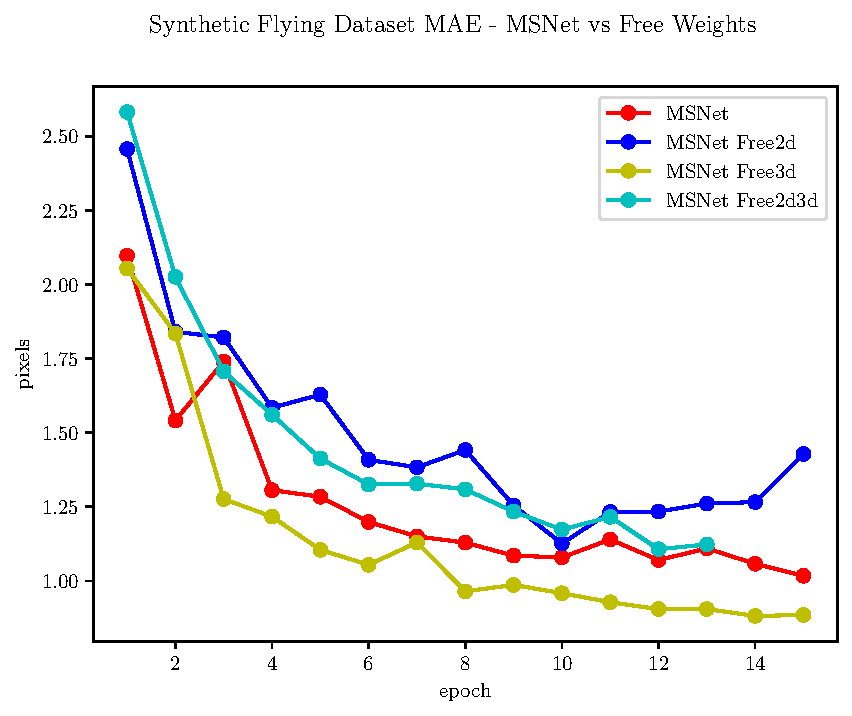
\includegraphics[width=0.49\textwidth]{figures/freiburg_msnet_vs_free_weights_mae.pdf}
    \caption{(Left) Comparison of MSNet with IMS architectures. (Right) Comparison of MSNet with Free Weight Networks.}
    \label{fig:mae_SFNvsGenericNets}
\end{figure}

\subsection{What Is the Cost of Sharing Weights}

MSNet is based on the idea of repeating its building blocks $f_1, f_2, f_3, f_4$ along the different scales. Following this principle, it obtains the crucial advantage of being adjustable to the application needs. An important question that arises is how much is the cost in terms of accuracy for gaining such scalability; what would be the corresponding end-point-error (EPE) if we were to apply the backbone architecture of MSNET without weight sharing (i.e. without repeating the same building blocks). For answering this question, we create a second internal benchmark, by implementing three new CNN architectures; MSNet Free2d has free weights only in the 2D-processing part (doesn't repeat $f_1$ blocks), MSNet Free3D has free weights only in the 3D-processing part (doesn't repeat $f_2, f_3, f_4$ building blocks) and, finally, MSNet Free2D3D has free weights everywhere. The results in the SceneFlow dataset are presented in figure \ref{fig:mae_SFNvsGenericNets} and in table \ref{tab:results}. We observe that repeating the 3D-processing building blocks ($f_2, f_3, f_4$) through the MultiScaleFusion algorithm leads to a suboptimal solution. Even though MSNet Free3D outperforms our proposed model, such approach cancels the scalability advantage of MSNet and is much more memory-intensive.

\subsection{MSNet vs State-Of-The-Art models}

In table \ref{tab:results}, we can compare the proposed MSNet model with the other SOTA architectures that have been proposed, in the SceneFlow dataset. We observe that MSNet achieves competitive performance (i.e. $1.017$ px of EPE compared to the $0.74$ in \cite{du2019amnet}) even though it uses much less free parameters ($0.7M$ compared to $4.37M$ parameters). This indicates that repeating building blocks along different scales is a beneficial designing principle, that can lead to competitive performance with smaller networks.  

\subsection{MSNet evaluation on different scale combinations}

The fundamental advantage of MSNet compared to other architectures is being able to be tuned between accuracy and efficiency at test time. In figure \ref{fig:msnet_scales_evaluation}, we measure how much the EPE of MSNet varies under using different scales. Firstly, we observe that the EPE and PCG error decreases as we add more scales. Additionaly, the standard deviation $\sigma$ of both EPE and PCG error gets smaller as we add more processing scales, which indicates that by operetaning in more scales we also gain robustness. In general terms adding coarse scales increases the robustness of our predictions, even though the mean EPE may be worse; for example $T=\{ 8 \}$ is better than $ T = \{ 16 \}$ in terms of EPE (i.e. smaller $\mu$ absolute error) but $ T = \{ 16 \}$ has smaller $\sigma$. 

\begin{figure}[htbp!]
    \centering
    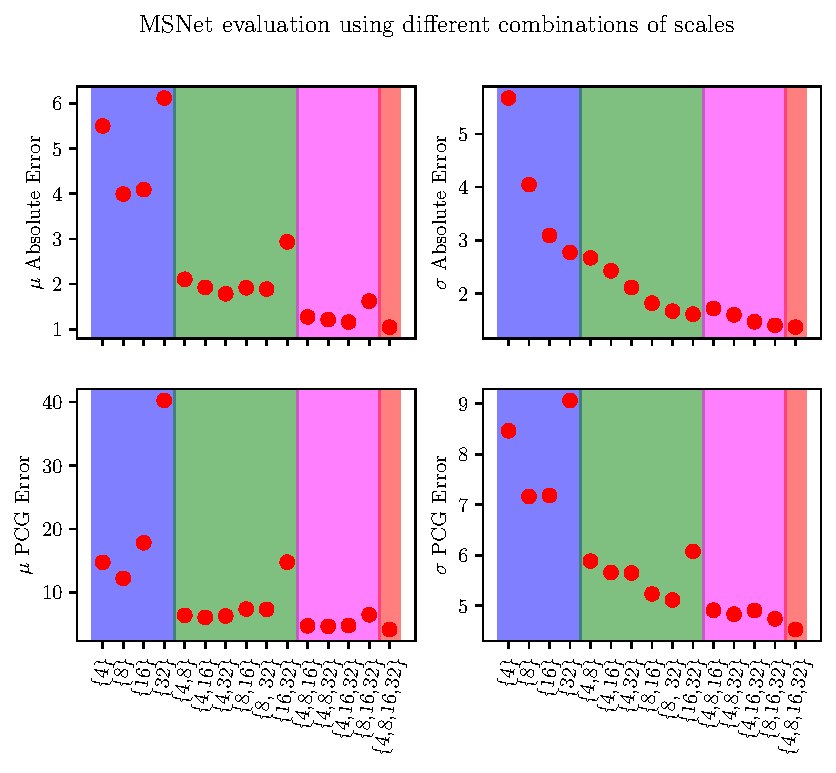
\includegraphics[width=0.6\textwidth]{figures/msnet_scales_evaluation.pdf}
    \caption{MSNet accuracy for different scale combinations. On the x-axis, there are the different scale combinations (i.e. the blue area contains single-scale set-ups, the green area two-scale, the purple area three-scale and the orange area the four-scale combination that was used in the training phase). On the first row we observe the $\mu$ and $\sigma$ of the absolute end-point error and on the second row the $\mu$ and $\sigma$ of the percentage of points with end-point error over 3 pixel.}
    \label{fig:msnet_scales_evaluation}
\end{figure}

\subsection{Multi-Scale fusion analysis} \label{sec:4_1}

In figure \ref{fig:multiscale_importance}, we show how our 3D cnn network has learned incorporating and progressively adopting fine scale predictions. We choose two points with different features; the yellow-box region contains a thin object with texture, which is appropriate for small and high-resolution patch. On the other hand, the orange-box contains a background wall with repetitive pattern, which needs a broader patch containing features from neighbourhood objects. In the orange-box scenario a small, high-resolution patch would lead to a confusion with each neighboor points. For confirming this hypothesis, we initially tune the network for single-scale predictions (i.e. right column in the graph). We can confirm that fine scale works well in the yellow-box and coarse scale in the orange-box region. On the left column, we observe the corresponding results, when the network is set to multi-scale prediction; it achieves accurate predictions in both cases, since it has learned to detect the appropriate scale and rely its prediction on it.

In figure \ref{fig:EMAPs} we present the predictions of the network along with the error images. We observe that initially, at the coarse scale, the network predicts a rough estimation of the depth without many details. As it operates through finer scales, it gradually adopts high-resolution details. This procedure can be seen, as a step-by-step refinement of the initial low-resolution prediction.

\begin{figure}[htbp!]
    \begin{center}
        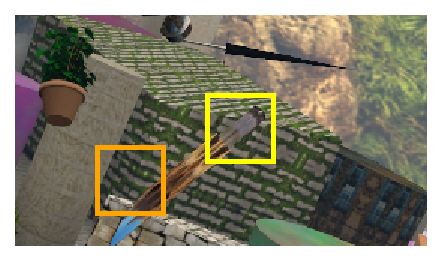
\includegraphics[width=0.49\textwidth]{paper/latex/figures/multiscale_importance_image_patches.pdf}\\
        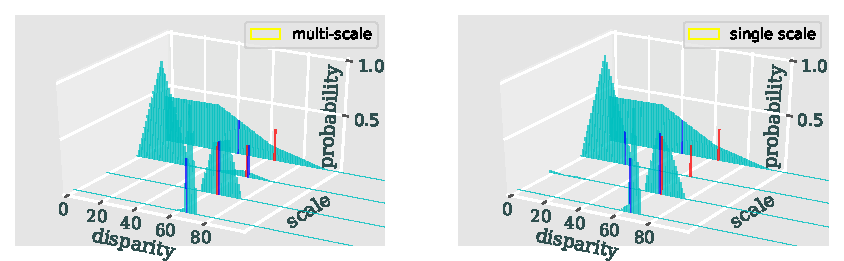
\includegraphics[width=0.75\textwidth]{paper/latex/figures/multiscale_importance_graph_high_resolution.pdf}\\
        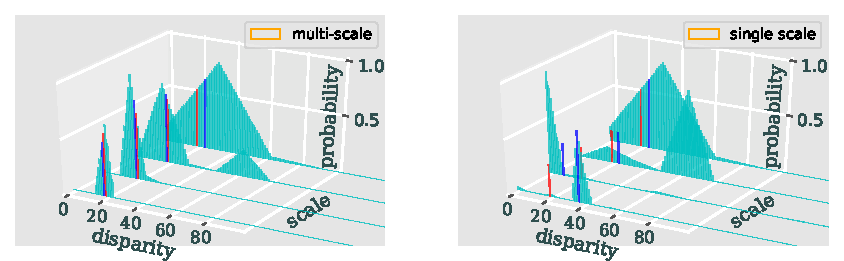
\includegraphics[width=0.75\textwidth]{figures/multiscale_importance_graph_low_resolution.pdf}
    \end{center}
    
    \caption{In this figure, we compare two regions of the same image that require processing on different scale. The centre point of the yellow rectangle is a small object on the foreground with many features (i.e. handle of a knife), whilst the orange one represents a background area inside a repetitive pattern. The first column of graphs represents the Multi-Scale similarity volumes $S^{\{ \sigma_0, ..., \sigma_n \} }$ The graphs prove that, as we expected, disparity estimation is accurate on higher scale for the yellow rectangle and on t As expected,  }
    \label{fig:multiscale_importance}
\end{figure}


\subsection{MSNet evaluation on smaller training set}

In figure \ref{fig:msnet_smaller_tr_set}, we present MSNet performance under training set of different size. As expected, the accuracy increases as the model observes more training data.

\begin{figure}[htbp!]
    \centering
    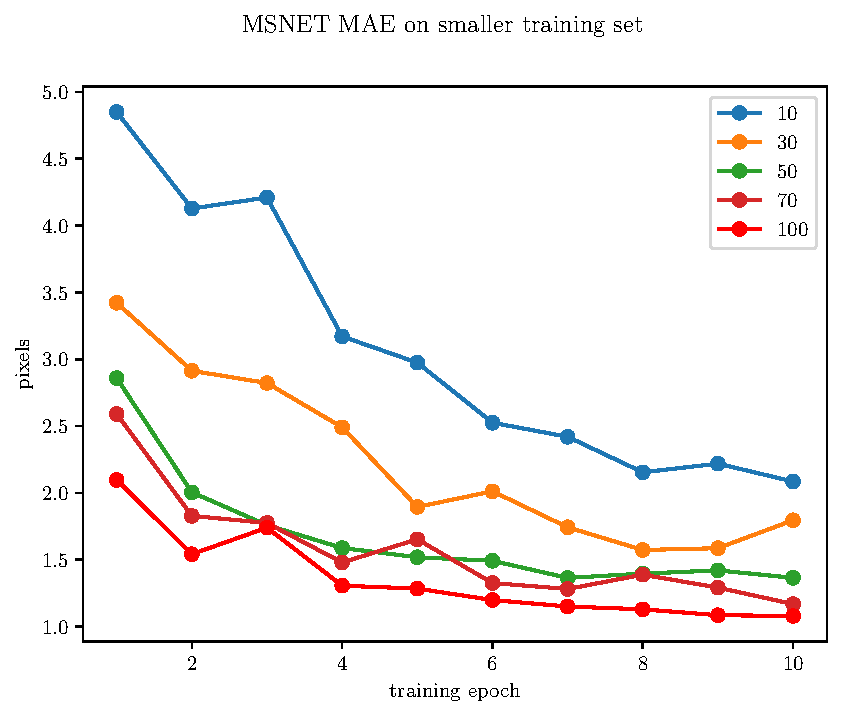
\includegraphics[width=0.45\textwidth]{figures/freiburg_msnet_mae_smaller_training_set.pdf}
    \caption{Caption}
    \label{fig:msnet_smaller_tr_set}
\end{figure}

\section{Conclusion and Future Work}

In this paper we proposed a scalable CNN, that can be adjusted to the needs of each application; it can be tuned for efficiency or accuracy, without finetuning. For achieving this agility, we exploited the key ideas of multiscale analysis, by training a processing module once and then apply it along the different scales.  We also saw that designing a CNN architecture that explicitly enforces multiscale processing, leads to superior performance by using less learnable parameters. Our method exhibits competitive results compared to the State-of-the-art methods in the SceneFlow dataset, even though it is a much smaller network.

Still, there are some open questions to be examined in the future. Firstly, as we explored experimentally, our recursive method for incorporating information from all different scales, even though it is fundamental for keeping the model fully scalable, it is suboptimal in terms of accuracy. Furthermore, our method can be reformed in an unsupervised problem by ... Finally, search for the appropriate scale based on the properties of the image...   
\clearpage
\bibliographystyle{splncs}
\bibliography{egbib}
\end{document}
